\documentclass[a4paper, 12pt, english]{article}

\usepackage[utf8]{inputenc}
\usepackage{amsmath,amssymb}
\usepackage{graphicx}
\usepackage{subfig}
\usepackage[colorinlistoftodos]{todonotes}

\usepackage{indentfirst}
\usepackage{verbatim}
\usepackage{textcomp}
\usepackage{gensymb}

\usepackage{relsize}

\usepackage{lipsum}% http://ctan.org/pkg/lipsum
\usepackage{xcolor}% http://ctan.org/pkg/xcolor
\usepackage{xparse}% http://ctan.org/pkg/xparse
\NewDocumentCommand{\myrule}{O{1pt} O{2pt} O{black}}{%
  \par\nobreak % don't break a page here
  \kern\the\prevdepth % don't take into account the depth of the preceding line
  \kern#2 % space before the rule
  {\color{#3}\hrule height #1 width\hsize} % the rule
  \kern#2 % space after the rule
  \nointerlineskip % no additional space after the rule
}
\usepackage[section]{placeins}

\usepackage{booktabs}
\usepackage{colortbl}%
   \newcommand{\myrowcolour}{\rowcolor[gray]{0.925}}
   
\usepackage[obeyspaces]{url}
\usepackage{etoolbox}
\usepackage[colorlinks,citecolor=black,urlcolor=blue,bookmarks=false,hypertexnames=true]{hyperref} 

\usepackage{geometry}
\geometry{
	paper=a4paper, % Change to letterpaper for US letter
	inner=3cm, % Inner margin
	outer=3cm, % Outer margin
	bindingoffset=.5cm, % Binding offset
	top=2cm, % Top margin
	bottom=2cm, % Bottom margin
	%showframe, % Uncomment to show how the type block is set on the page
}

\usepackage{float}

\usepackage{amsmath,amsfonts}


\usepackage{multicol,caption}
\newenvironment{Figure}
  {\par\medskip\noindent\minipage{\linewidth}}
  {\endminipage\par\medskip}
\usepackage{array}

\usepackage{listings}
% MATLAB code formatting
\lstdefinestyle{matlab}{
    language=Matlab,
    basicstyle=\scriptsize\ttfamily,
    keywordstyle=\color{blue},
    commentstyle=\color{green!40!black},
    stringstyle=\color{red},
    showstringspaces=false,
    numbers=left,
    numberstyle=\tiny,
    numbersep=5pt,
    tabsize=2,
    breaklines=true,
    breakatwhitespace=true
}
% MATLAB command window formatting
\lstdefinestyle{commandstyle}{
    basicstyle=\scriptsize\ttfamily,
    numbers=none,
    showstringspaces=false,
    breaklines=true,
    frame=single,
    frameround=fttt,
    backgroundcolor=\color{gray!10},
    xleftmargin=0.5cm,
    xrightmargin=0.5cm
}

\newcommand{\highlight}[1]{\textcolor{blue}{\texttt{#1}}}

\usepackage[backend=biber, style=ieee]{biblatex}
\addbibresource{references.bib}

\graphicspath{{images/}}

\setlength {\marginparwidth }{2cm} 

\newcommand{\usection}[1]{\section*{#1}
\addcontentsline{toc}{section}{\protect\numberline{}#1}}

\newcommand{\usubsection}[1]{\subsection*{#1}
\addcontentsline{toc}{subsection}{\protect\numberline{}#1}}

\newcommand{\usubsubsection}[1]{\subsubsection*{#1}
\addcontentsline{toc}{subsubsection}{\protect\numberline{}#1}}

\usepackage{bm}
%*******************************************************************************%
%************************************START**************************************%
%*******************************************************************************%
\begin{document}

%************************************TITLE PAGE**************************************%
\begin{titlepage}
\begin{center}
\textbf{\LARGE Alexandria University}\\[0.5cm] 
\textbf{\large FACULTY OF ENGINEERING}\\[0.2cm]
\vspace{20pt}

\includegraphics{logo.png}\\[1cm]
\par
\vspace{20pt}
\textbf{\Large EEC471 Automatic Control Systems}\\
\vspace{15pt}
\myrule[1pt][7pt]
\textbf{\LARGE  Lab Assignment 1}\\
\vspace{15pt}
\textbf{\large Hybrid Electric Vehicles (HEV)}\\
\myrule[1pt][7pt]
\vspace{25pt}
\textbf{\large \hspace{50pt}Student Name \hspace{60pt} Student ID}\\
Ahmed Osama Mohamed Afifi \hspace{60pt} 20010038 \\

\vspace{45pt}
%\textbf {\large Lecturer in charge:}\\[0.2cm]
%\Large {Dr. Lorem Ipsum}\\[0.1cm]
\end{center}

\par
\vfill
\begin{center}
\textbf{Submission Date : 27/10/2024}\\
\end{center}

\end{titlepage}

%************************************TABLE OF CONTENTS**************************************%

%  %Summary
  \newpage
  \hypersetup{linkcolor=black}
  \tableofcontents
%  \thispagestyle{empty}
  %End Summary

%********************************%
%***********SECTION 1************%
%********************************%
\newpage
\section{Introduction}
This report presents the work conducted in Lab Assignment 1, which focuses on the fundamental concepts of block diagrams, block diagram reduction, and transfer functions. The lab specifically addresses the use of these techniques to model, simplify, and analyze the control systems that govern the operation of Hybrid Electric Vehicles (HEVs). By applying block diagram reduction methods, complex control systems in HEVs can be simplified for easier analysis and design, aiding in the efficient management of both electric and internal combustion power sources.
\begin{figure}[H]
    \centering
    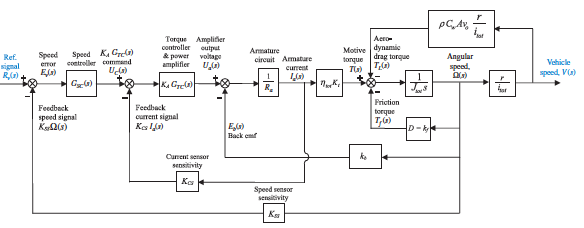
\includegraphics[width=\linewidth]{images/hev.png}
    \caption{Block diagram of a control scheme for an HEV driven by a DC motor}
    \label{fig:Block diagram of a control scheme for an HEV driven by a DC motor}
\end{figure}
%********************************%
%***********SECTION 2************%
%********************************%
\section{Simulink}
The block diagram in Figure \ref{fig:Block diagram of a control scheme for an HEV driven by a DC motor} was converted into a Simulink model, as shown in Figure \ref{fig:Simulink block diagram}. This conversion allows for simulation-based analysis
\begin{figure}[H]
    \centering
    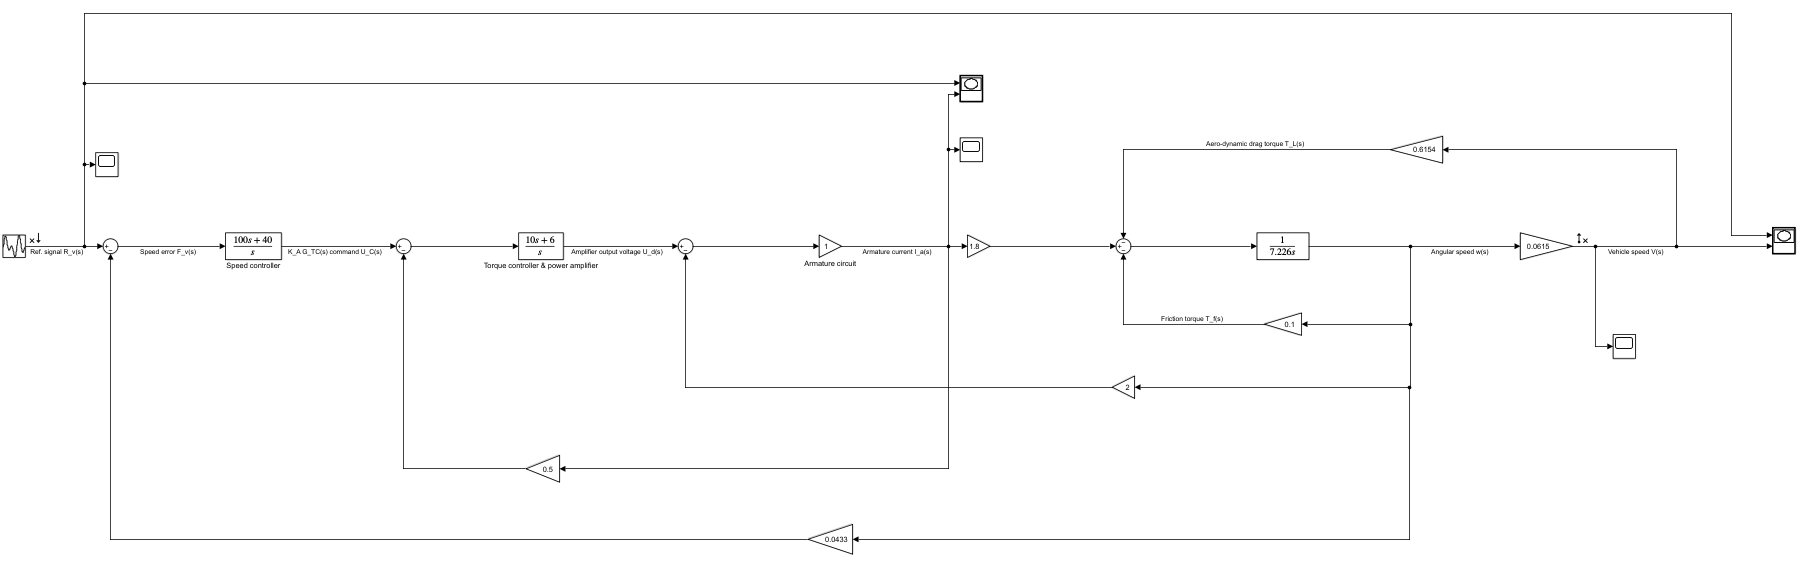
\includegraphics[width=\linewidth]{images/simulink.png}
    \caption{Simulink block diagram}
    \label{fig:Simulink block diagram}
\end{figure}

\subsection{Input}
As specified in the lab instructions, for IDs ending in 8, a square wave input with an amplitude of 5, frequency of 5 Hz, phase angle of 0, and an 80\% duty cycle was used.
\begin{figure}[H]
    \centering
    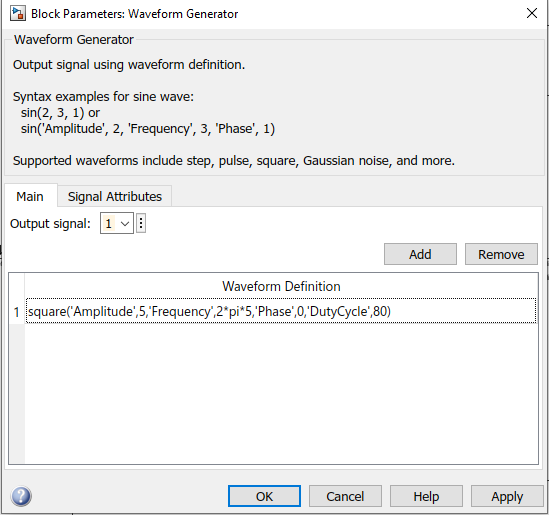
\includegraphics[width=0.5\linewidth]{images/input.png}
    \caption{Input signal characteristics}
    \label{fig:Input signal characteristics}
\end{figure}
\begin{figure}[H]
    \centering
    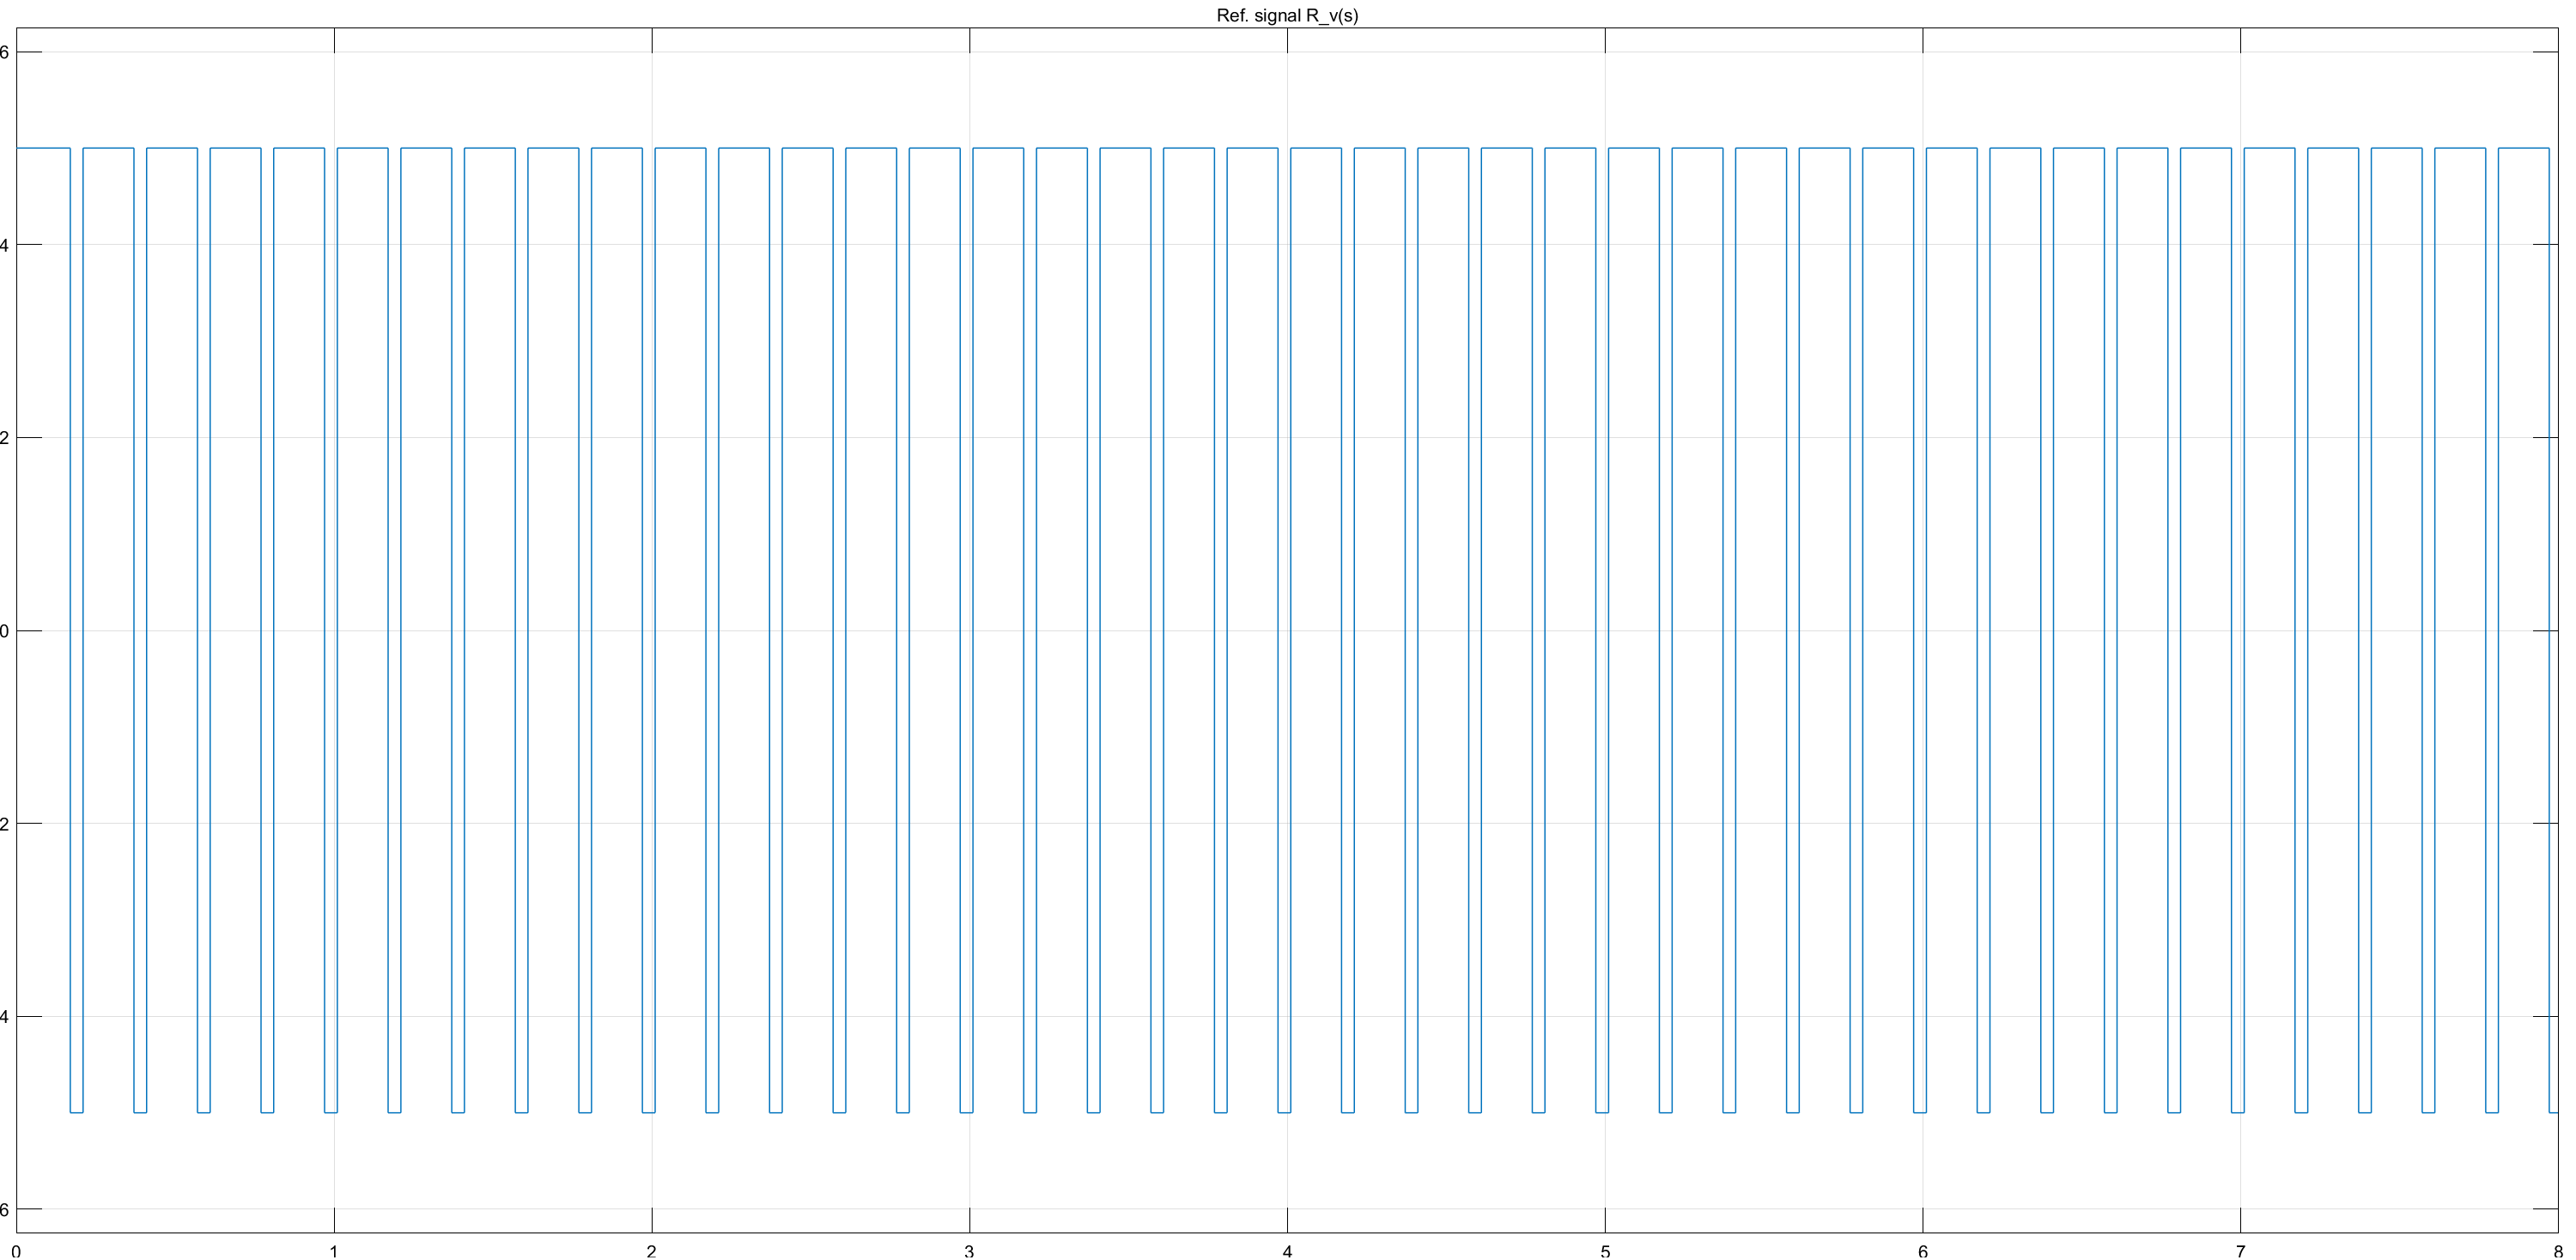
\includegraphics[width=\linewidth]{images/input_signal.png}
    \caption{Input signal}
    \label{fig:Input signal}
\end{figure}

\subsection{Output}
The resulting vehicle speed output is shown, reflecting the system’s response to the applied square wave input.
\begin{figure}[H]
    \centering
    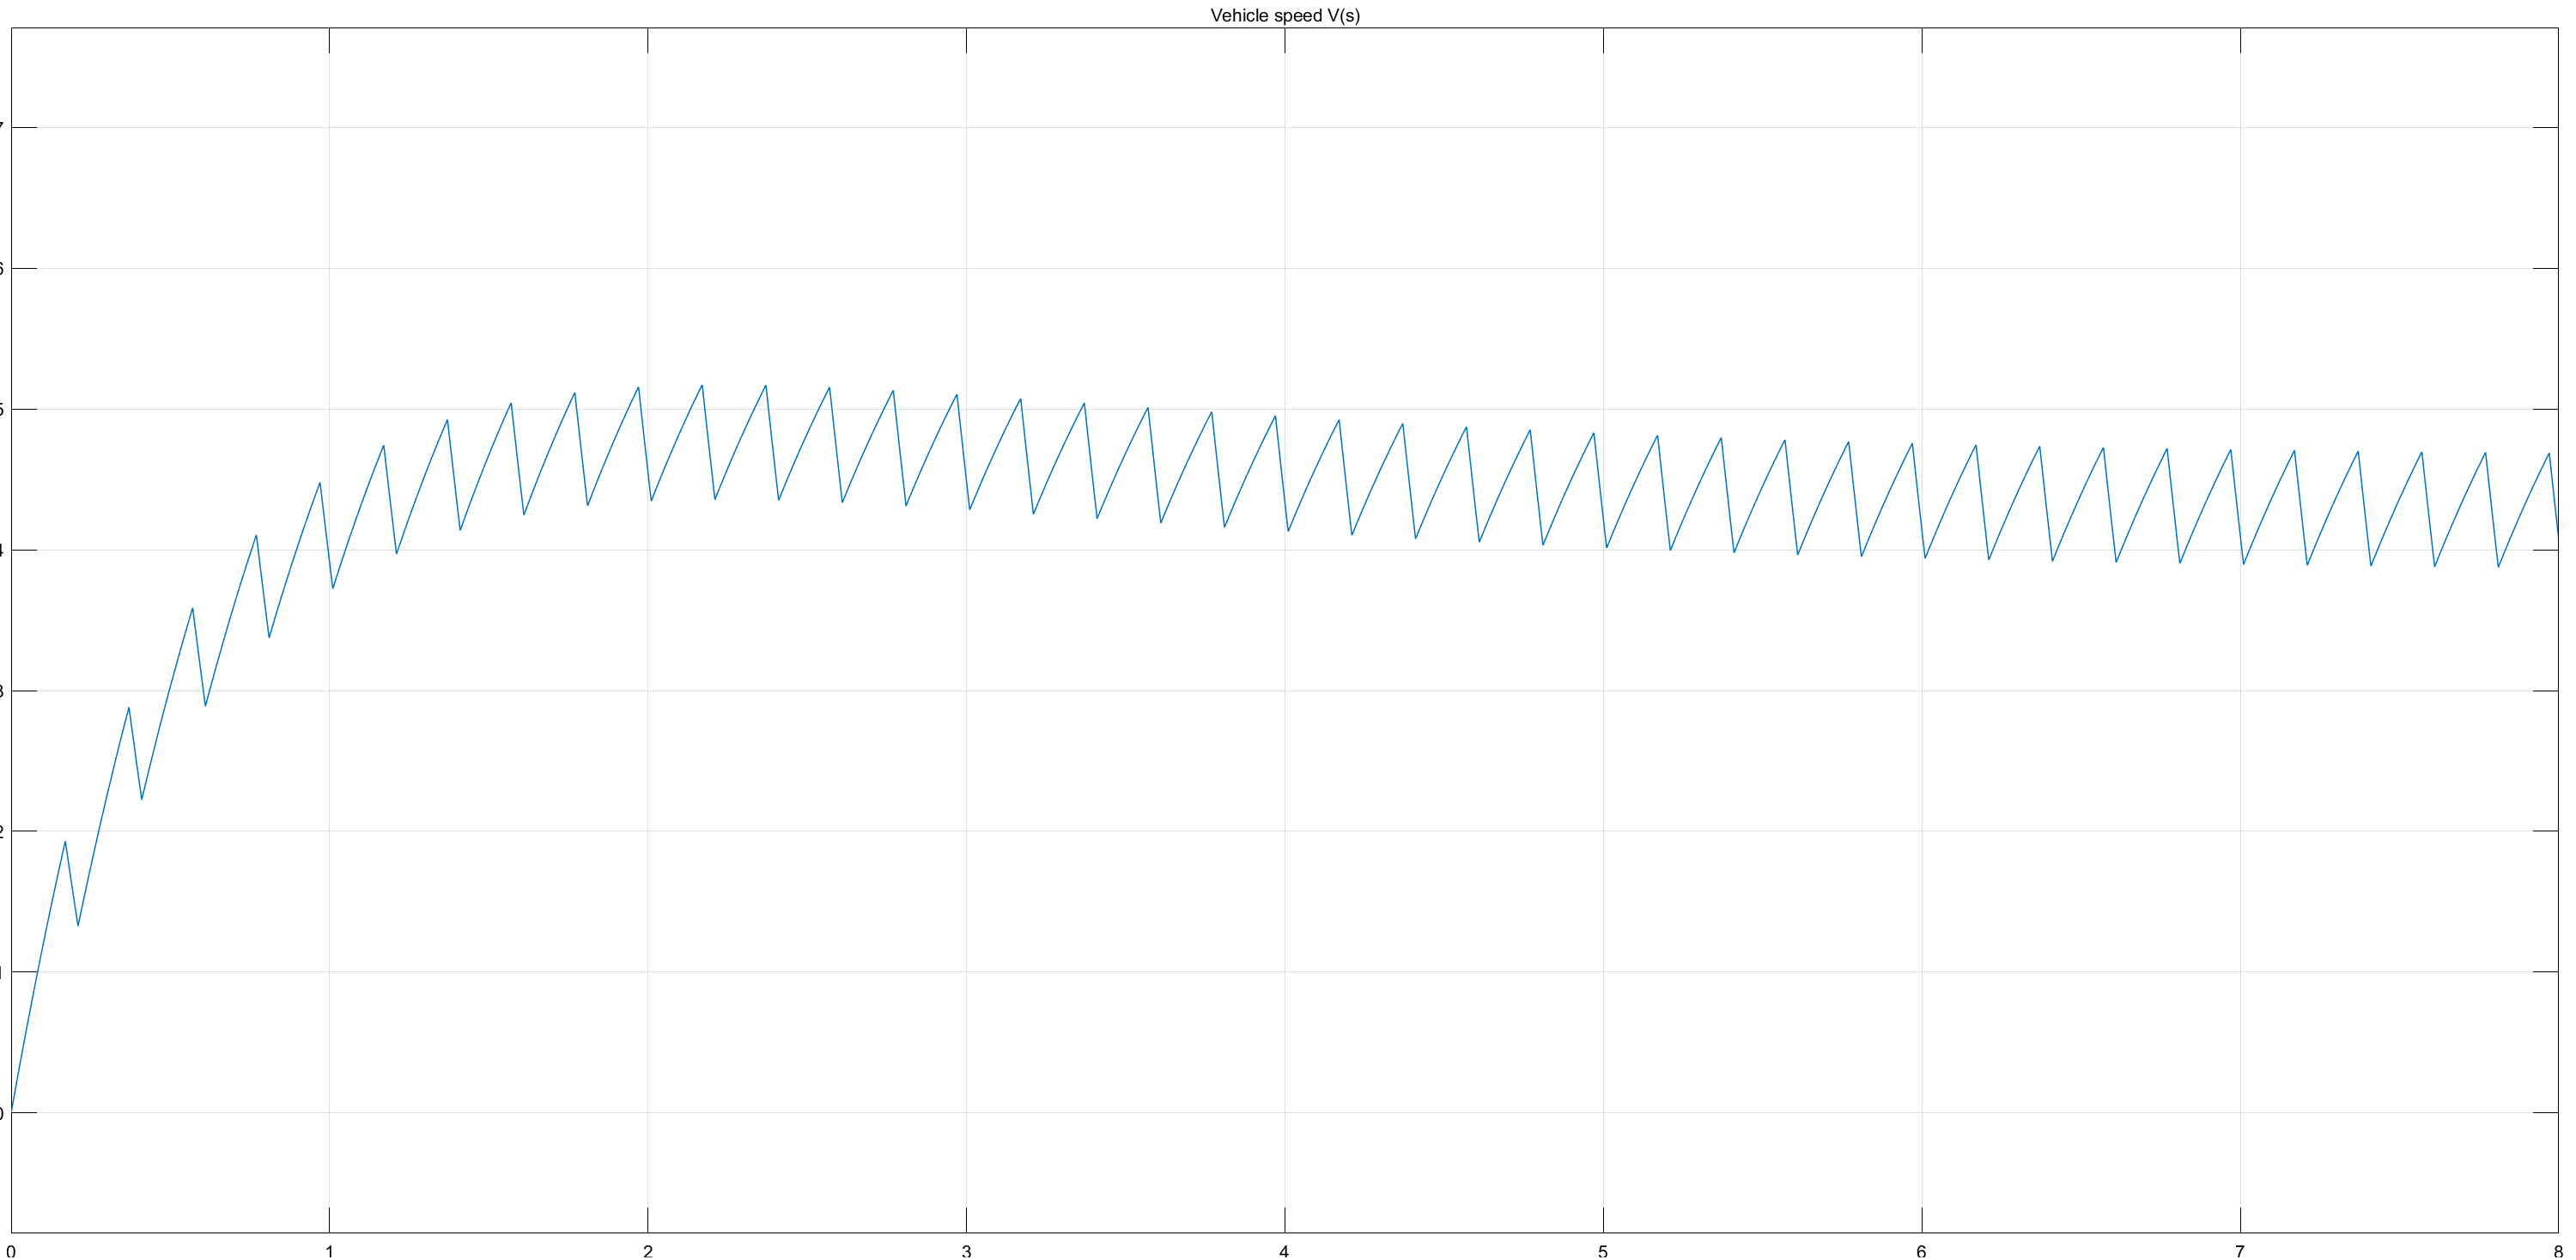
\includegraphics[width=\linewidth]{images/vehicle_speed.png}
    \caption{Vehicle speed signal}
    \label{fig:Vehicle speed signal}
\end{figure}

The resulting motor armature current is shown, reflecting the system’s response to the applied square wave input.
\begin{figure}[H]
    \centering
    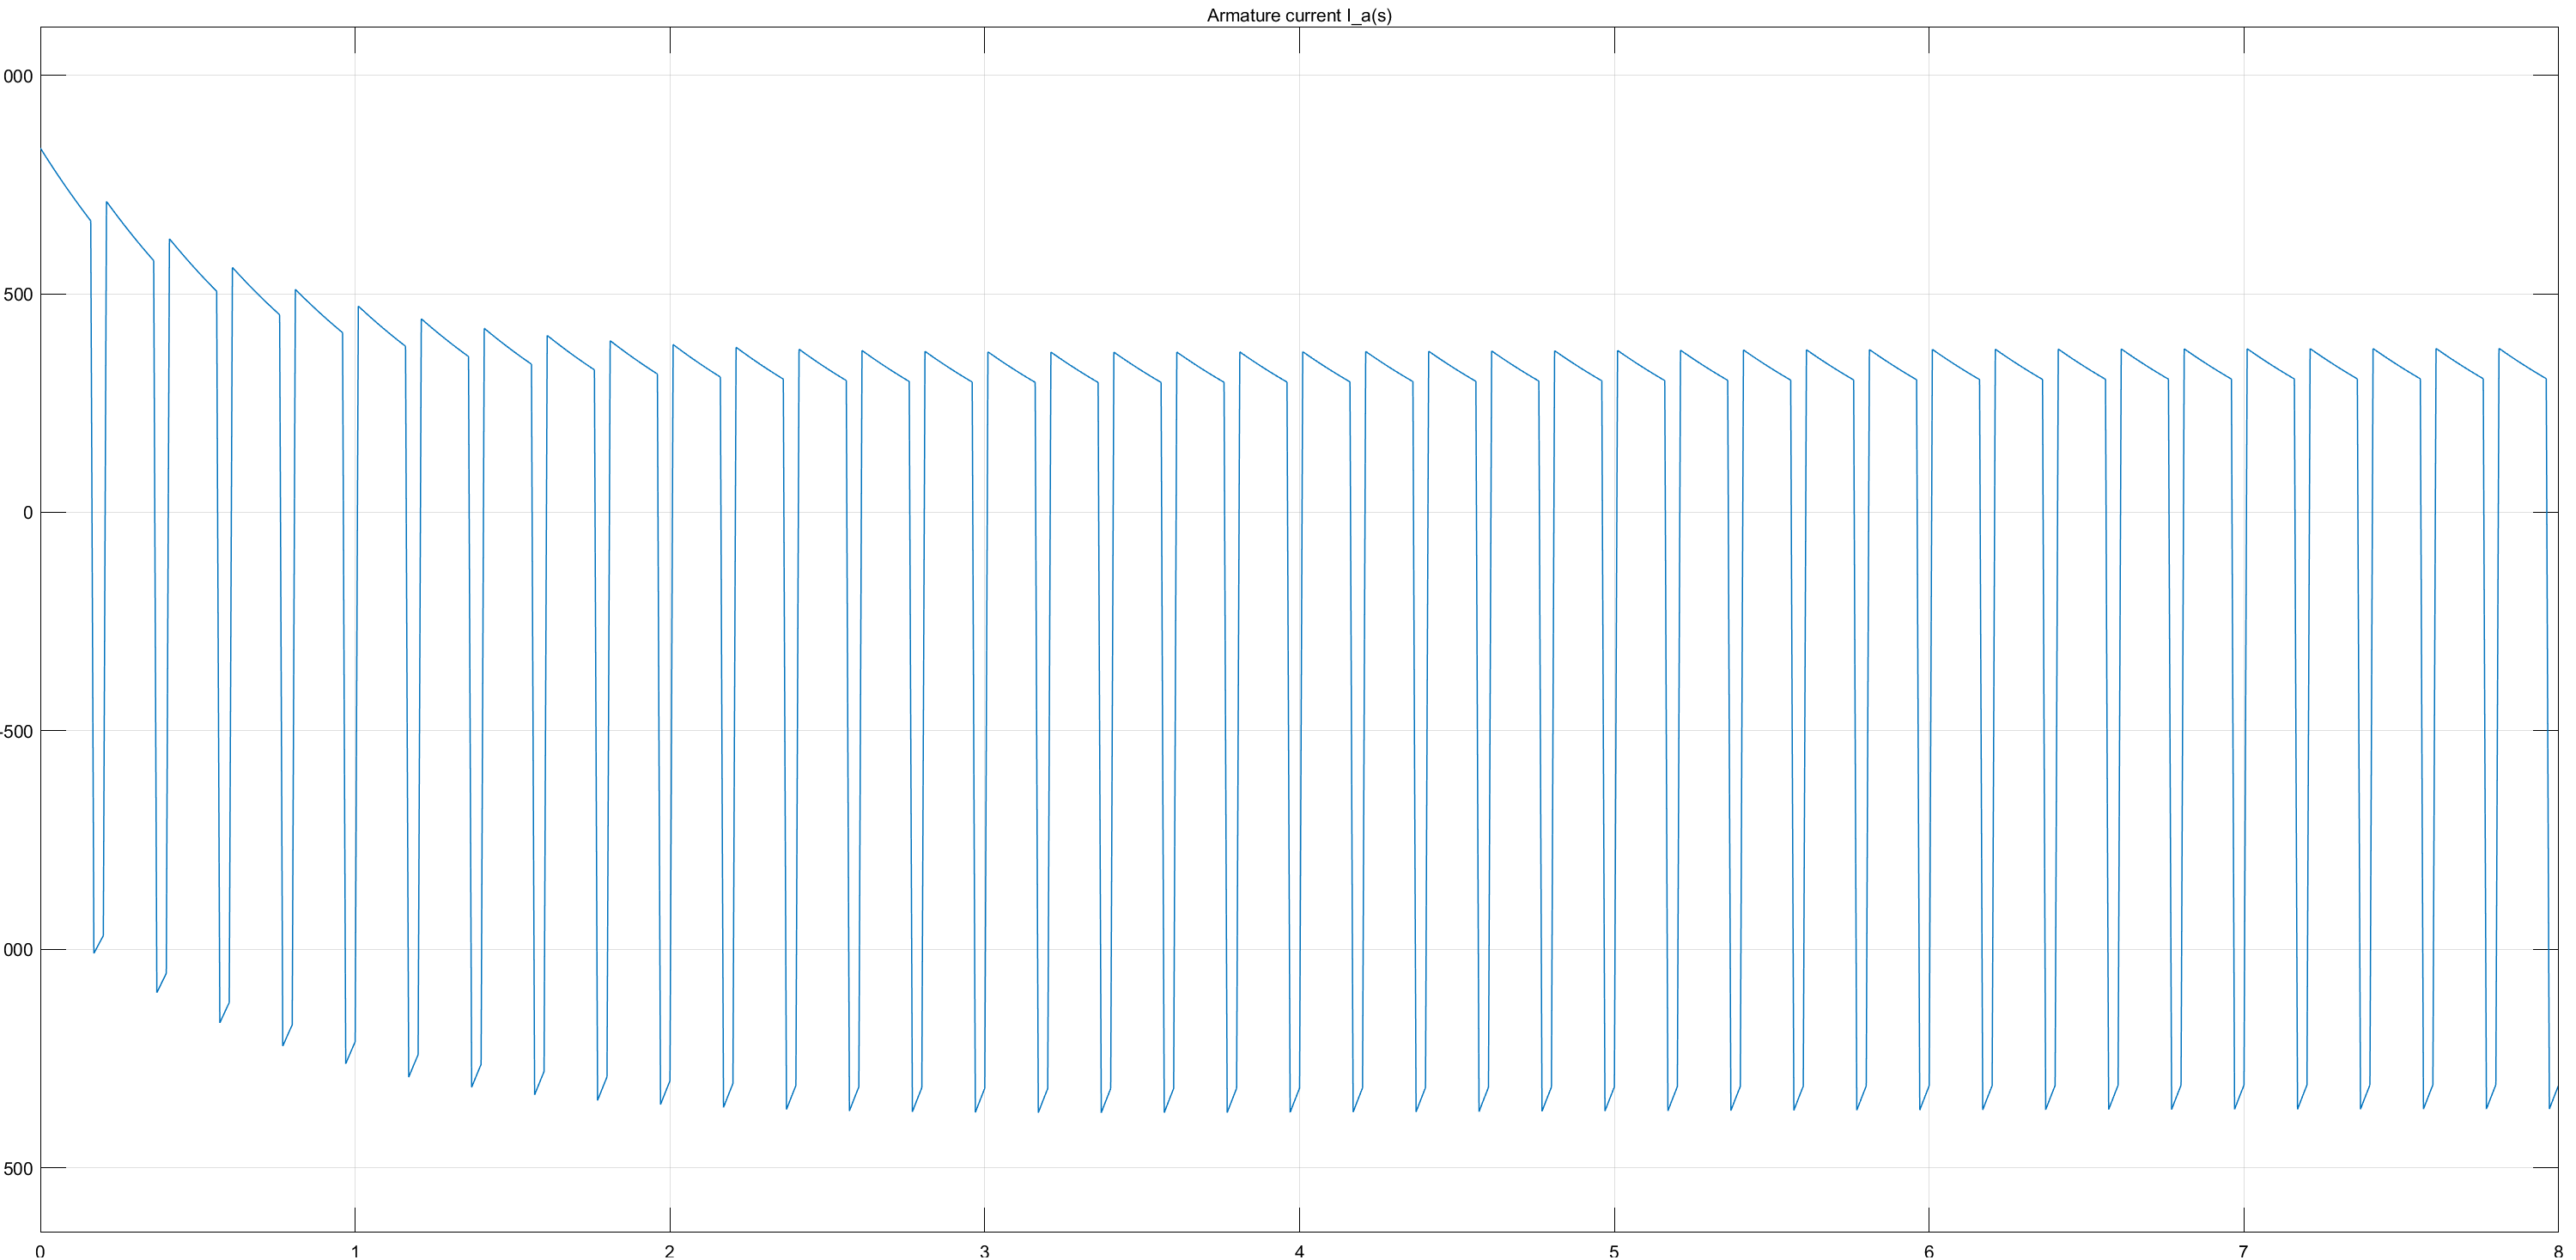
\includegraphics[width=\linewidth]{images/armature_current.png}
    \caption{Motor armature current signal}
    \label{fig:Motor armature current signal}
\end{figure}

The speed versus input signal graph illustrates the relationship between the square wave input and the resulting vehicle speed output.
\begin{figure}[H]
    \centering
    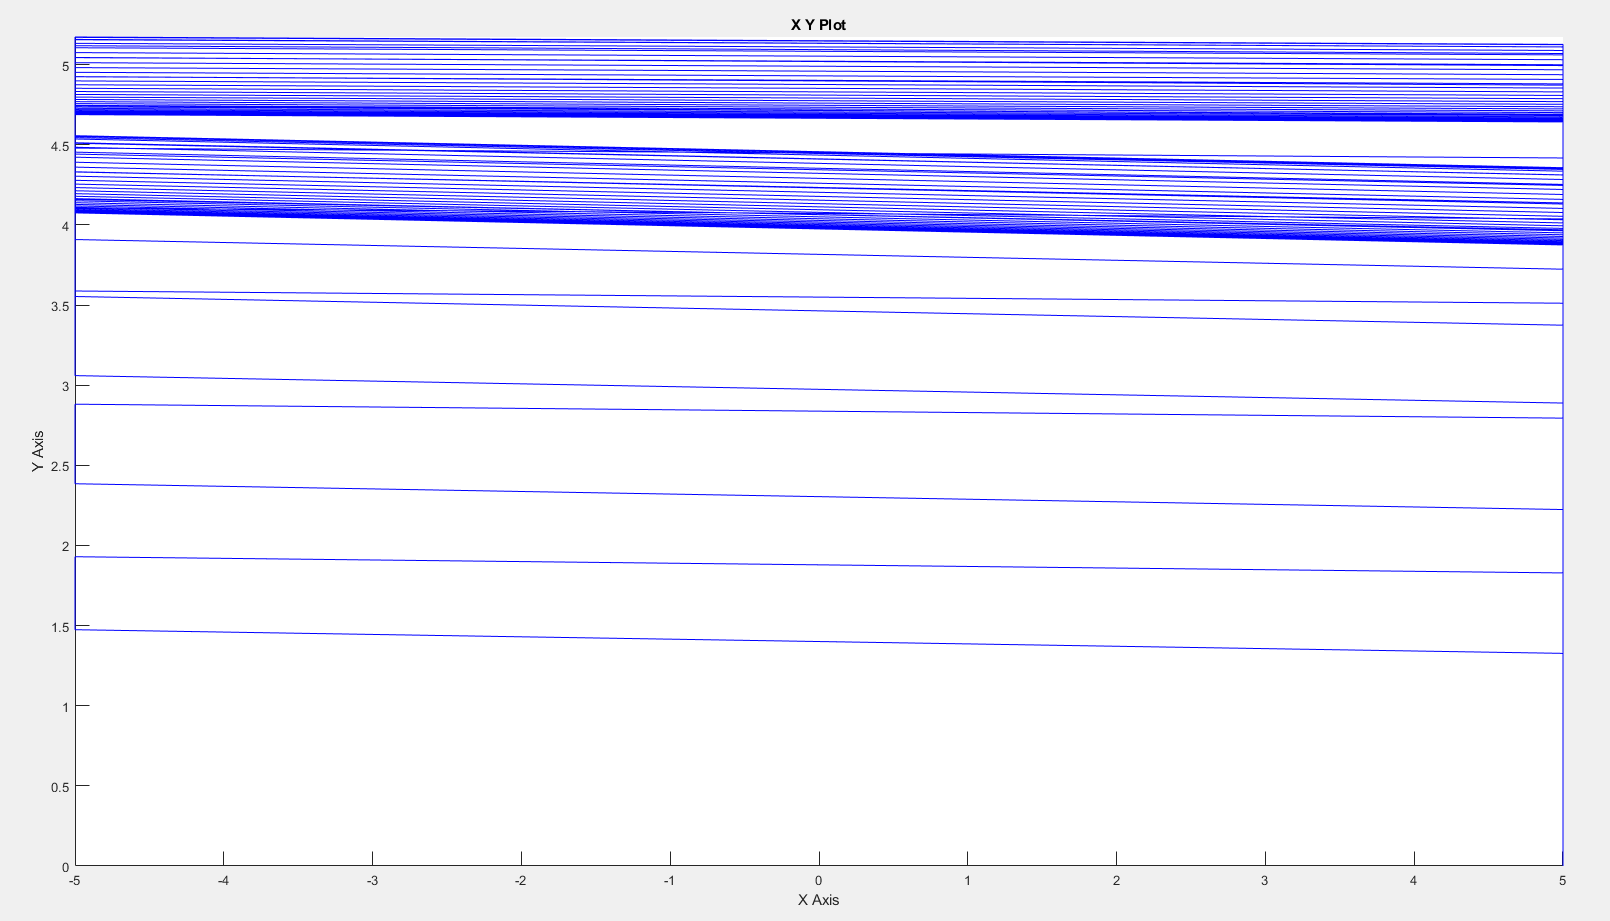
\includegraphics[width=\linewidth]{images/speed_input.png}
    \caption{Vehicle speed versus input signal}
    \label{fig:Vehicle speed versus input signal}
\end{figure}

The motor armature current versus input signal graph illustrates the relationship between the square wave input and the resulting motor armature current output.
\begin{figure}[H]
    \centering
    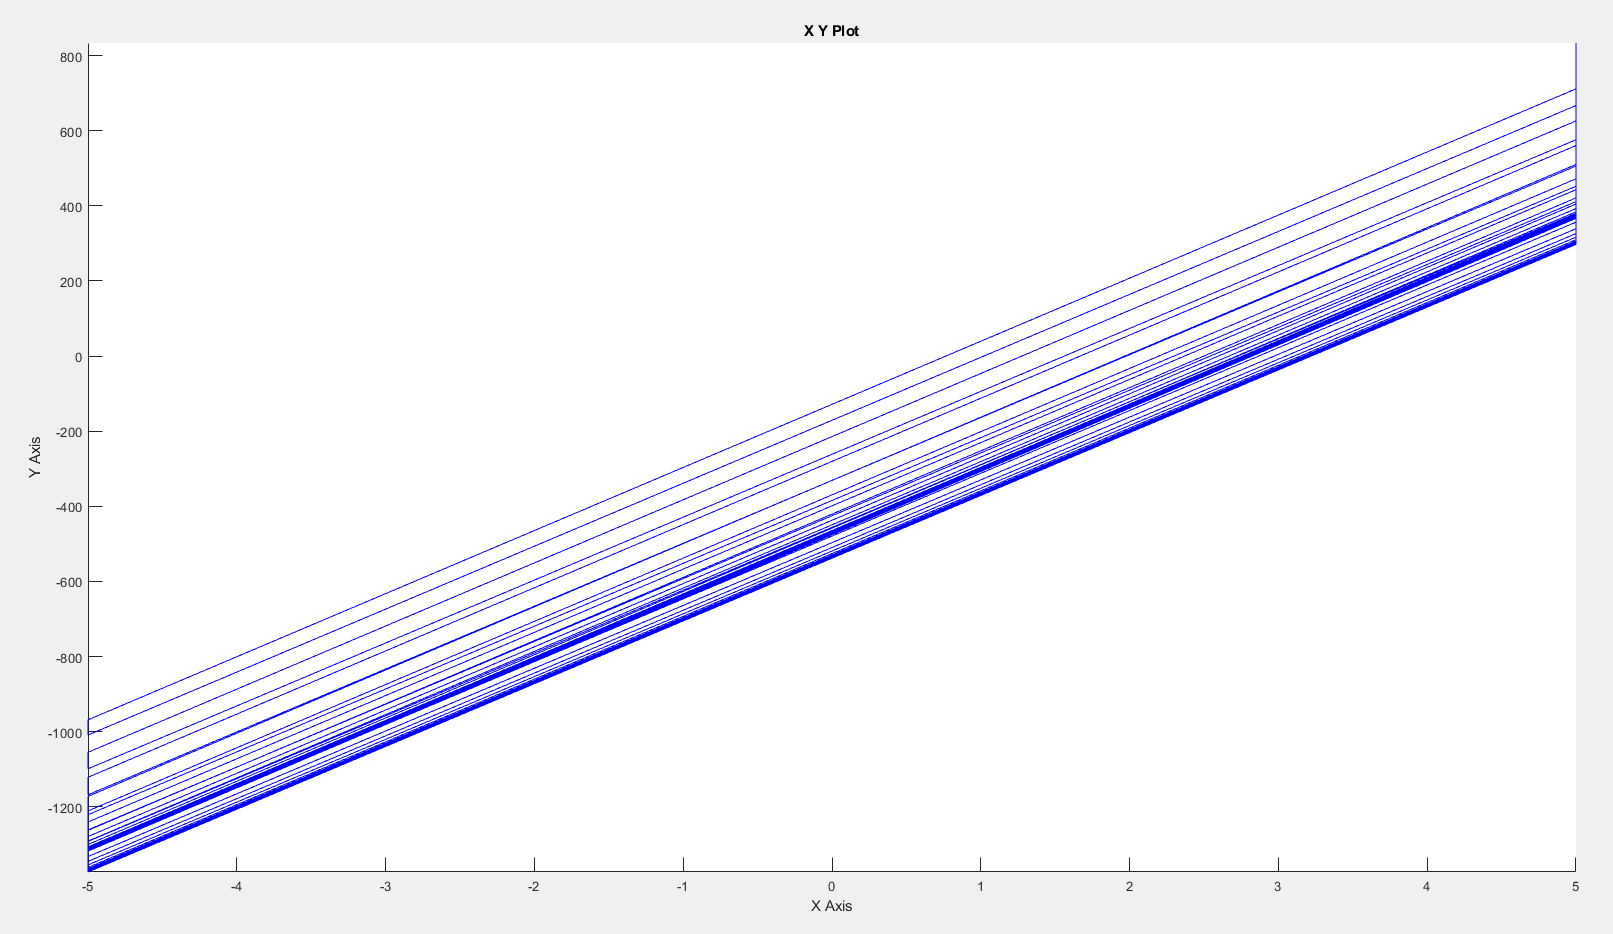
\includegraphics[width=\linewidth]{images/current_input.png}
    \caption{Motor armature current versus input signal}
    \label{fig:Motor armature current versus input signal}
\end{figure}

\subsection{Transfer function}
The transfer function of the HEV control system was measured in Simulink using the model linearization tool, applying an impulse response for analysis. This method allows for the characterization of the system's dynamic behavior by observing its response to a sudden input change, which is essential for understanding the system's stability and response characteristics.

By applying an impulse input, the system's output response was recorded, enabling the extraction of the transfer function that relates the input to the output in the frequency domain. This transfer function provides critical insights into the system's poles and zeros, which are fundamental for assessing system stability, transient response, and overall performance. \\
\newline
The linearization tool in Simulink streamlines this process, automatically computing the transfer function based on the observed input-output data.
\begin{figure}[H]
    \centering
    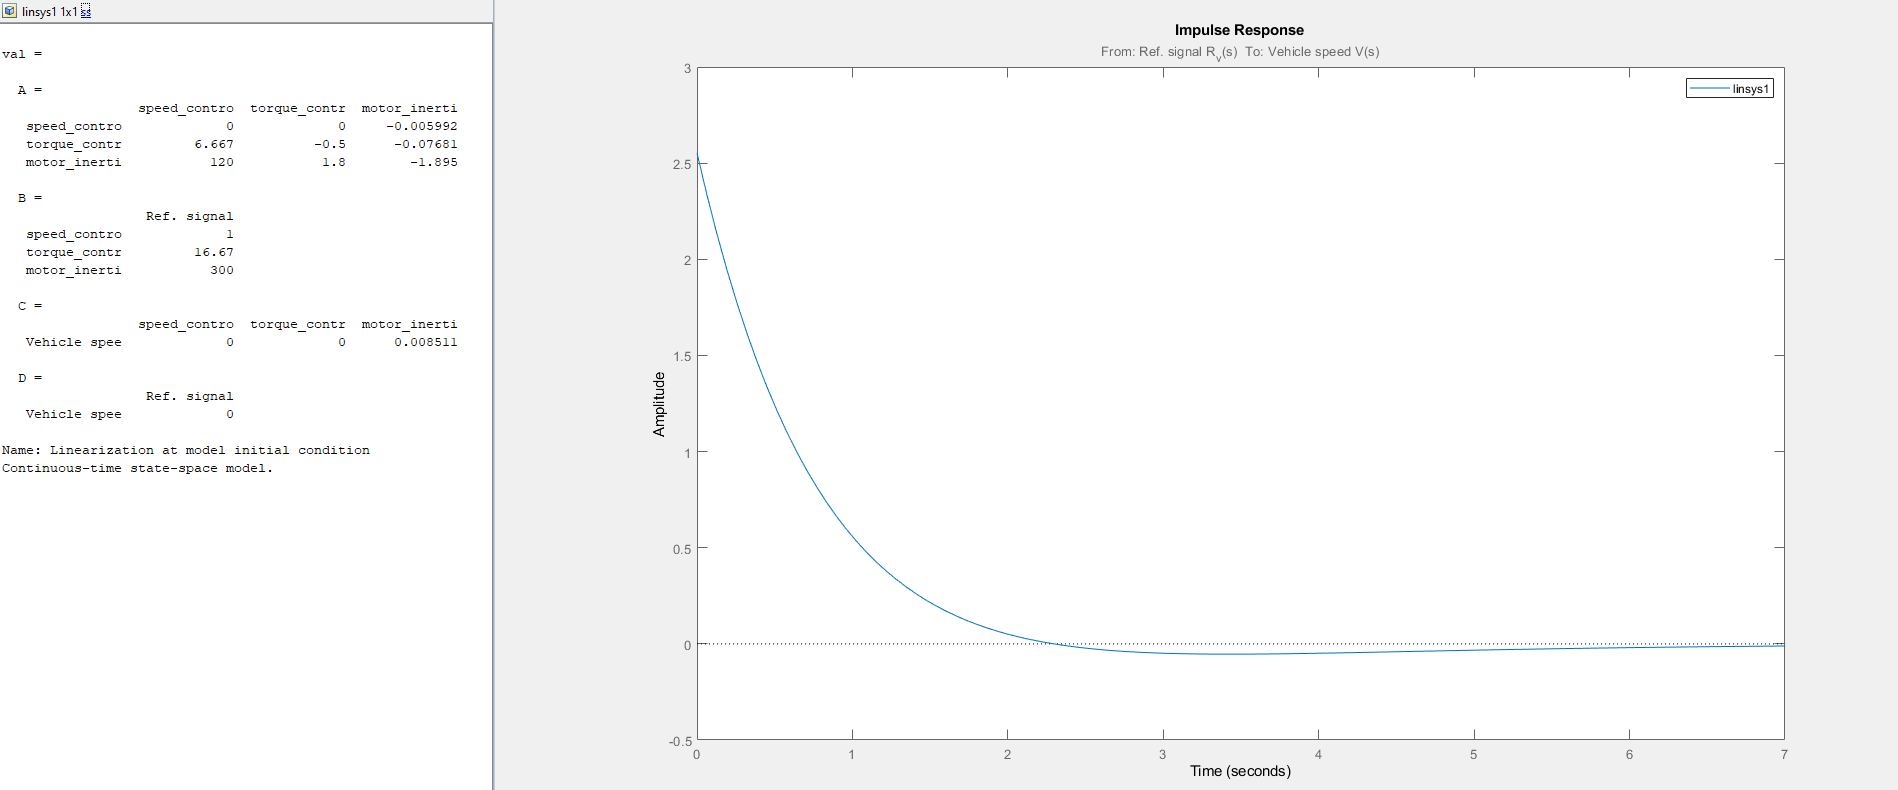
\includegraphics[width=\linewidth]{images/impulse_response.png}
    \caption{Impulse response}
    \label{fig:Impulse response}
\end{figure}

\begin{lstlisting}[style=commandstyle,caption={Transfer function},captionpos=b]
>> tf(LinearAnalysisToolProject.Results.Data.Value)

ans =
 
  From input "Ref. signal R_v(s)" to output "Vehicle speed V(s)":
     2.553 s^2 + 2.553 s + 0.6128
  ----------------------------------
  s^3 + 2.395 s^2 + 1.805 s + 0.4314
 
Name: Linearization at model initial condition
Continuous-time transfer function.
\end{lstlisting} 

%********************************%
%***********SECTION 3************%
%********************************%
\section{Matlab}

In the MATLAB implementation, each component of the HEV control system is represented as transfer functions, beginning with the speed controller and torque controller, as shown in lines 1 to 11 of the code. \\

The subsequent reduction process, detailed in lines 13 to 25, combines these elements to simplify the overall control system. Each stage of the reduction builds upon the previous one, utilizing feedback and series connections to create an integrated model of the HEV system.\\

Finally, the transfer function of the entire HEV system is calculated in lines 27 and 28. The `tfdata` function extracts the numerator and denominator of the overall transfer function, which is then normalized to provide a more straightforward representation. The resulting transfer function, displayed for analysis, encapsulates the dynamic characteristics of the HEV control system, facilitating further study and optimization of its performance. \\
\begin{lstlisting}[style=matlab,caption={Matlab code},captionpos=b]
speed_ctrl = tf([100 40], [1 0]);               % Speed Controller
trq_ctrl = tf([10 6], [1 0]);                   % Torque Controller
motor_inertia = tf(1, [7.226 0]);               % Motor Inertia
K_cs = 0.5;                                     % Current Sensor Senstivity
K_ss = 0.0433;                                  % Speed Sensor Senstivity
k_f = 0.1;                                      % Viscous friction
k_b = 2;                                        % Back EMF constant
R_a = 1;                                        % Motor Resistance
motor_trq = 1.8;                                % Motor torque
vehicle_trq = 0.6154;                           % Vehicle torque
vehicle_speed = 0.0615;                         % Vehile speed

stage1 = feedback(motor_inertia, k_f);
k_b = k_b / vehicle_speed;
K_ss = K_ss / vehicle_speed;
stage2 = series(stage1, vehicle_speed);
stage3 = feedback(stage2, vehicle_trq);
stage4 = series(motor_trq, stage3);
K_cs = K_cs / stage4;
stage5 = series((1/R_a), stage4);
stage6 = feedback(stage5, k_b);
stage7 = series(trq_ctrl, stage6);
stage8 = feedback(stage7, K_cs);
stage9 = series(speed_ctrl, stage8);
hev = feedback(stage9, K_ss);

[num, den] = tfdata(hev);
transfere_function = tf(num{1}/den{1}(1), den{1}/den{1}(1));
display(transfere_function);
\end{lstlisting}

\begin{lstlisting}[style=commandstyle,caption={Transfer function},captionpos=b]
>> lab1_code

transfere_function =
 
    2.553 s^2 + 2.553 s + 0.6128
  --------------------------------
  s^3 + 2.4 s^2 + 1.807 s + 0.4314
 
Continuous-time transfer function.
\end{lstlisting}

It is observed that the transfer function calculated from Simulink matches the one derived from MATLAB, confirming the consistency and accuracy of the modeling process. This correlation indicates that both environments accurately capture the dynamics of the HEV control system, providing reliable representations for analysis and design.

\section{Conclusion}
In this lab assignment, we successfully explored the fundamental concepts of block diagrams, block diagram reduction, and transfer functions within the context of Hybrid Electric Vehicles (HEVs). By converting a block diagram into a Simulink model, we gained valuable insights into the dynamic behavior of the control system, allowing us to analyze the system's response to a square wave input effectively. \\

The results demonstrated a clear relationship between the input signal and both the vehicle speed and motor armature current outputs, providing a practical understanding of how the control system manages operational demands. The measurement of the transfer function using Simulink's model linearization tool further validated our analysis, revealing consistent results between the Simulink and MATLAB computations.

\end{document}